%TEX root = ../dissertation.tex

\chapter{User Interface Contextualisation}
\label{chapter:user_interface}

The first step in successfully analysing the digital image is to specify the exact location of each masses nucleus or calcifications nucleus. The image is projected onto a computer screen, and the clinical medical operator uses, preferentially, a mouse button that will trace a rough outline of each visible masses (Figure 4.1) nucleus. On the other hand, the clinical medical operator will mark with dots the calcification (Figure 4.2) nucleus of cells.

For a precise and rigorous diagnosis of the cancer in mammography, it is necessary a successful step when analysing the image, specifying the exact location and morphology of the masses as well as calcifications.

% Commands to include a figure:
\begin{figure}[!hbt]
\centering
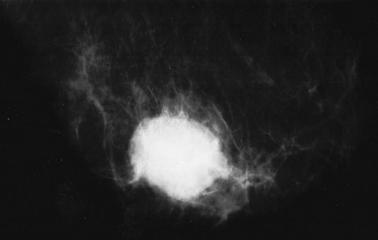
\includegraphics[width=15cm]{images/masses}~\\
\caption{\label{fig:frog}Mammographic image of a high-density mass
}
\end{figure}

% Commands to include a figure:
\begin{figure}[!hbt]
\centering
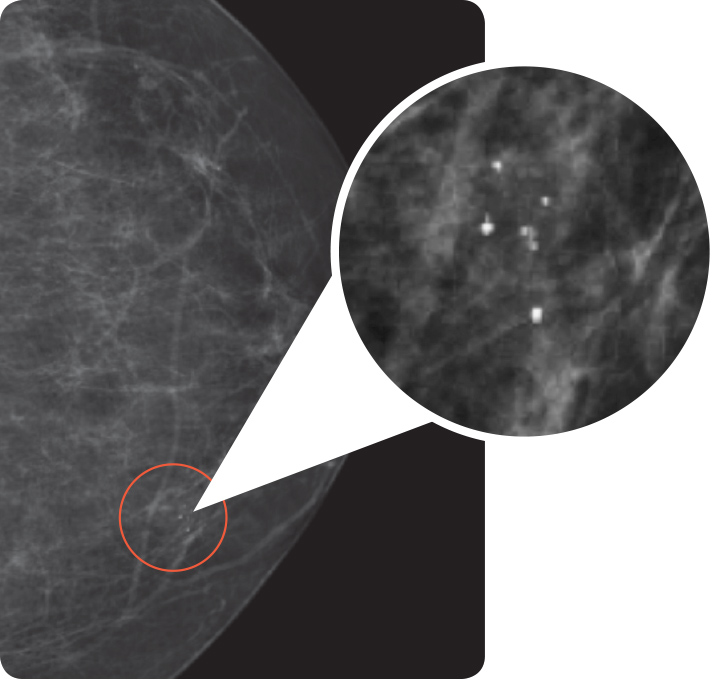
\includegraphics[width=15cm]{images/calcifications}~\\
\caption{\label{fig:frog}Mammogram – shows calcifications, an early sign of breast cancer
}
\end{figure}